\documentclass[a4paper,11pt]{article}
\usepackage[utf8]{inputenc}
\usepackage[ngerman]{babel}
\usepackage{geometry}
\geometry{left=25mm, top=20mm, right=25mm, headheight=14pt}
\usepackage[onehalfspacing]{setspace}
\usepackage{graphicx}
\usepackage{indentfirst}
\usepackage{lastpage}
\usepackage{pdfpages}
\usepackage{listings}
\usepackage{textcomp}
\usepackage{xcolor}
\usepackage{hyperref}

\newcommand*{\mybox}[2]{\colorbox{#1!30}{\parbox{.98\linewidth}{#2}}}
\hypersetup{
	colorlinks,
	citecolor=black,
	filecolor=black,
	linkcolor=black,
	urlcolor=black
}


\definecolor{background}{gray}{0.5}
\newcommand{\code}[1]{\colorbox{background}{\texttt{#1}}}

\lstset{ basicstyle=\small\ttfamily }
\lstset{
	backgroundcolor = \color{background}
,
	numbers=left,
	breaklines=true
}
\lstset{literate=%
	{Ö}{{\"O}}1
	{Ä}{{\"A}}1
	{Ü}{{\"U}}1
	{ß}{{\ss}}1
	{ü}{{\"u}}1
	{ä}{{\"a}}1
	{ö}{{\"o}}1
}


\pagenumbering{arabic}


\newcommand{\sign}[1]{%
	\begin{tabular}[t]{@{}l@{}}
		\makebox[2in]{\dotfill}\\
		\strut#1\strut
	\end{tabular}%
}

\begin{document}
\begin{titlepage}
	\hfill
	\vfill
	{
	\begin{center}
	\huge{\textbf{Entwicklung eines Softwaresystems 2019}}
	---------\\
	\large{\textbf{Landkartenerstellung}}
	\end{center}
	}

	\vfill
{\textit{\\Vorgelegt von:\\}}
	{Christoph Schirmel\\}
	{Pr\"ufungsnummer: }
	{101-20510\\}
	{Ausbildungsbetrieb: }
	{CAE Elektronik GmbH}
\end{titlepage}
\tableofcontents
\newpage

\includepdf{ErklaerungUnterschrieben.pdf}
{\parindent0pt
\section{Aufgabenbeschreibung}
Die MATSEgraphic AG stellt den Auftrag zur Erstellung von schemenhaften Karten auf Basis vorgegebener Kennwerte. Ausgangspunkt ist eine gegebene Menge an beliebigen Staaten mit
ihrer realen Lage, angegeben in L\"aengen- und Breitengrad, ihren realen Nachbarschaftsbeziehungen und dem jeweiligen Kennwert. Die Staaten sollen auf der erstellten Karte als Kreis
dargestellt werden. Die Gr\"oesse des Kreises ist proportional zu der gegebenen Kenngr\"oesse, also wird der Kreis f\"ur gr\"oessere Kennwerte gr\"oesser und f\"ur kleinere Kennwerte kleiner.
In der erstellten Karte sollen die Lage- und Nachbarschaftsbeziehungen so gut wie m\"oglich erhalten bleiben. Die Qualit\"at der Karte bemisst sich insgesamt am Abstand der L\"ander zueinander, sowie den Lage-
und Nachbarschaftsbeziehungen. \"Uberschneidungen und zu grosse Abst\"ande mindern die Qualit\"at der Karte und sollen vermieden werden. Die numerische Gr\"ossenordnung der Karte kann beliebig skaliert werden und hat keinen 
unmittelbaren Einfluss auf die Qualit\"at der Karte, welche lediglich durch die oben beschriebenen Kriterien bestimmt wird.

\vspace{10mm}
\textbf{Beispiel:}

\begin{center}
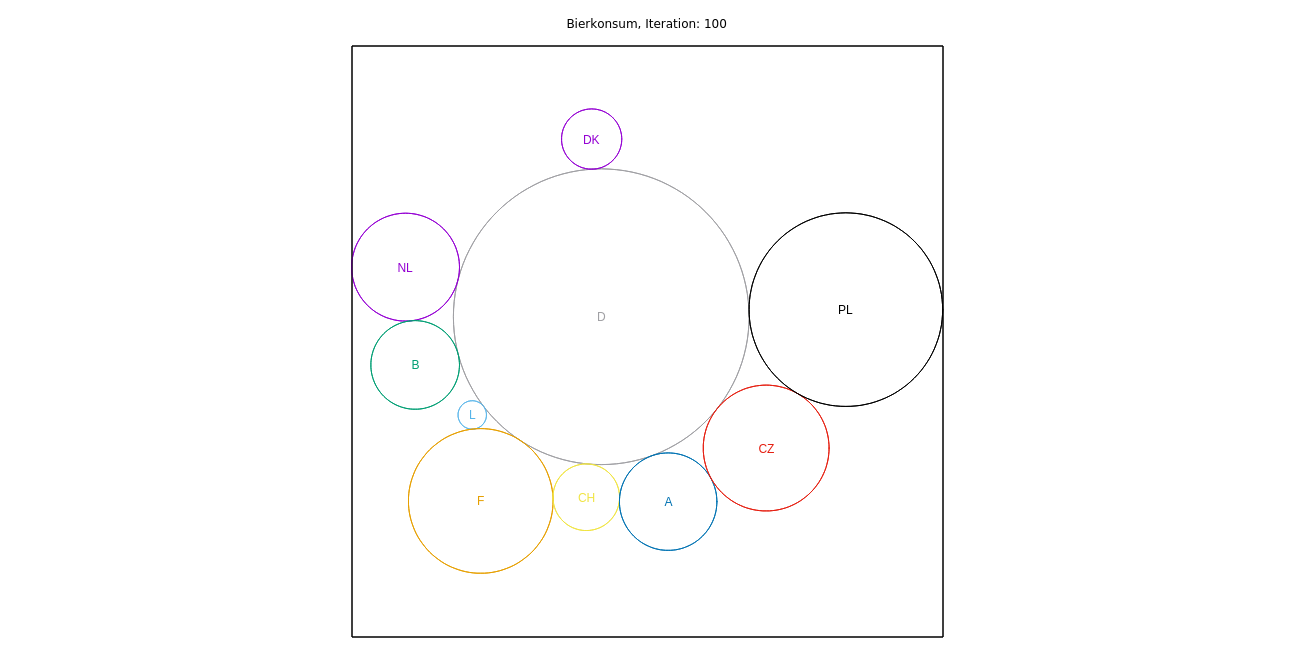
\includegraphics[width=\linewidth]{ihk_beispiel2.png}
\end{center}

Das obige Beispiel zeigt eine schematische Darstellung Mitteleuropas mit Deutschland und seinen Nachbarstaaten. Der Kennwert ist der Bierkonsum der einzelnen Staaten. Erkennbar ist, dass die Staaten nicht im Verh\"altnis
ihrer Fl\"ache sondern zum Kennwert dargestellt werden.
\subsection{Eingabedatei}
Zur Erstellung der Landkarte sollen \"uber eine Eingabedatei Daten eingelesen werden. Die Datei hat folgendes Format:
Die erste Zeile enth\"alt den Titel der Karte, z.B. "Fl\"ache der Staaten".
Zeilen, die mit "\#" beginnen, sind Kommentare und werden im weiteren Ablauf nicht betrachtet.
Nach dem ersten Kommentar folgen alle Staaten zeilenweise mit jeweils einem Staat pro Zeile. Dabei enth\"alt jede Zeile die folgenden Informationen:
\begin{itemize}
\item Autokennzeichen, z.B. "D" f\"ur Deutschland
\item Kennzahl
\item L\"angengrad
\item Breitengrad
\end{itemize}
Die Informationen sind jeweils durch Whitespace, Tab oder Leerzeichen, getrennt.
Auf die Liste der Staaten folgt ein Kommentar mit dem Hinweis, dass im Anschluss die Nachbarschaftsbeziehungen folgen. Jene folgen ebenfalls zeilenweise.
Die Nachbarschaftsbeziehungen werden bidirektional angegeben, d.h. ist ein Staat A ein Nachbar von Staat B, so ist automatisch auch B Nachbar von A.
Das Format der Nachbarschaftsbeziehungen sieht wie folgt aus:
\mybox{background}{$<$Kennz. Ausgangsland$>$: $<$Kennzeichen Nachbar 1$>$ $<$...$>$ $<$Kennzeichen Nachbar N$>$}
Die einzelnen Nachbarstaaten sind ebenfalls durch Whitespace (Leerzeichen oder Tab) getrennt. 
Grundsätzlich wird angenommen, dass das Format der Eingabedatei syntaktisch korrekt ist. Die Syntax wird daher nicht mehr auf Korrektheit \"uberpr\"uft.

\vspace{10mm}

\textbf{Beispiel:}\\
Die Eingabedatei vom vorherigen Beispiel k\"onnte wie folgt aussehen:\\
\vspace{5mm}
\mybox{background}{
Bierkonsum\\
\# Staat Fläche Längengrad Breitengrad\\
D 8692 10.0 51.3\\
NL 1156 5.3 52.2\\
B 781 4.8 50.7\\
L 80 6.1 49.8\\
F 2077 2.8 47.4\\
CH 440 8.2 46.9\\
A 945 14.2 47.6\\
CZ 1573 15.3 49.8\\
PL 3724 18.9 52.2\\
DK 360 9.6 56.0\\
\# Nachbarschaften\\
D: NL B L F CH A CZ PL DK\\
NL: B\\
L: F\\
F: CH\\
CH: A\\
A: CZ\\
CZ: PL
}
\subsection{Ausgabedatei}
Nach dem Einlesen der oben beschriebenen Daten und der Berechnung der Landkarte soll eine Ausgabe mit den berechneten Werten erstellt werden.
Diese soll dem folgenden Format gen\"ugen:
\mybox{background}{
reset
set xrange [$<$xmin$>$:$<$xmax$>$]
set yrange [$<$ymin$>$:$<$ymax$>$]\\
set size ratio 1.0\\
set title "$<$Name des Kennwertes$>$, Iteration: $<$nr$>$"\\
unset xtics\\
unset ytics\\
\$data $<<$ EOD\\
$<$Liste aus $<$xpos$>$ $<$ypos$>$ $<$radius$>$ $<$autokennzeichen$>$ $<$id$>$ $>$\\
EOD\\
plot \textbackslash\\
'\$data' using 1:2:3:5 with circles lc var notitle, \textbackslash\\
'\$data' using 1:2:4:5 with labels font \grqq{}arial,9\grqq{}  tc variable notitle\\
}
\\
\\
Die Intervalle \colorbox{lightgray}{[$<$xmin$>$:$<$xmax$>$]} und \colorbox{lightgray}{[$<$ymin$>$:$<$ymax$>$]} geben jeweils die kleinste und gr\"osste x- bzw. y-Koordinate der Landkarte an.
\colorbox{lightgray}{$<$Name des Kennwertes$>$} gibt den Namen des Kennwertes an, der in der Eingabedatei in der 1. Zeile angegeben wird.
Die Anzahl der Iterationen wird in \colorbox{lightgray}{$<$nr$>$} angegeben.
In der \colorbox{lightgray}{$<$Liste aus $<$xpos$>$ $<$ypos$>$ $<$radius$>$ $<$autokennzeichen$>$ $<$id$>$ $>$} werden alle Staaten nacheinander aufgelistet. Die Werte
\colorbox{lightgray}{$<$xpos$>$ und $<$ypos$>$} sind die Koordinaten des jeweiligen Kreismittelpunktes, der \colorbox{lightgray}{$<$radius$>$} ist der ermittelte Radius des Kreises.
Das \colorbox{lightgray}{$<$autokennzeichen$>$} gibt das Kennzeichen des Staats an und die \colorbox{lightgray}{$<$id$>$} ist eine fortlaufende Nummerierung beginnend bei 0, die f\"ur die 
Farbgebung in Gnuplot erforderlich ist.\\
\vspace{40mm}\\
\textbf{Beispiel:}\\
\vbox{
Die Ausgabe f\"ur das Beispiel \glqq{}Bierkonsum\grqq{} k\"onnte wie folgt aussehen:\\
\mybox{background}{
reset\\
set xrange[122.2902588107926:332.4746754411094]\\
set yrange[990.7016847962033:1200.88610142652]\\
set size ratio 1.0\\
set title "Bierkonsum, Iteration: 100"\\
unset xtics\\
unset ytics\\
\$data << EOD\\
211.053730834 1104.45871827 52.5999004819 D 0\\
141.472704651 1122.09603019 19.1824458406 NL 1\\
144.871946688 1087.31207915 15.7670549282 B 2\\
165.183777819 1069.53934032 5.04626504404 L 3\\
168.191312507 1038.92448868 25.7124412222 F 4\\
205.719560567 1040.2435555 11.8345405454 CH 5\\
234.860729713 1038.69277989 17.3436686558 A 6\\
269.709149473 1057.75886679 22.3763591982 CZ 7\\
298.045240126 1106.99471738 34.4294353156 PL 8\\
207.661916065 1167.67099407 10.7047446969 DK 9\\
EOD\\
plot \textbackslash \\
'\$data' using 1:2:3:5 with circles lc var notitle, \textbackslash \\
'\$data' using 1:2:4:5 with labels font \grqq{}arial,9\grqq{} tc variable notitle\\
}
}
\subsection{Spezial- und Sonderf\"alle bei der Eingabe}
Syntaxfehler in der Eingabedatei sind laut Aufgabenstellung ausgeschlossen. Daher benutze ich als Format f\"ur meine Eingabedatei restriktiv das unter Punkt 1.1 angegebene Format,
inklusive der Kommentarzeilen.\\ Den Inhalt der Kommentarzeilen ignoriere ich, allerdings benutze ich sie zur Orientierung beim Einlesen der Zeilen. Vor dem ersten Kommentarzeichen, das ein \# ist, befindet sich
der Titel, auf den ersten Kommentar folgen die Staaten und nach dem zweiten Kommentar kommen die Nachbarschaftsbeziehungen.\\ \\ \textbf{Vorschriften}:\\
\vspace{3mm}
\begin{itemize}
\item Doppelt vorkommende Autokennzeichen sind nicht erlaubt, da diese eindeutig sein m\"ussen, um einen Staat eindeutig identifizieren zu k\"onnen.\\
\item Zwei mal der selbe Mittelpunkt f\"ur zwei verschiedene Staaten ist nicht erlaubt. \\
\item Der Kennwert muss mindestens 1 sein.
\item Kennwerte sollten nicht zu gross gew\"ahlt werden, weil das Koordinatensystem durch den gew\"ahlten Datentyp
double beschr\"ankt ist und es ansonsten in Ausnahmef\"allen durch die berechneten Kr\"afte zu einer \"Uberschreitung des erlaubten Wertebereichs kommen k\"onnte. In diesem Fall w\"are es erforderlich die Kennzahl anzupassen, bpsw. durch eine \"Anderung der Gr\"ossenordnung.
\item Die L\"angen- und Breitengrade m\"ussen im Wertebereich des \textit{World Geodetic System 1984 (WGS84)} liegen. Das bedeutet, dass die Breitengrade im Intervall [-90;+90] liegen m\"ussen und L\"angengrade im Intervall [-180;+180].
Andere Werte werden nicht akzeptiert.
\item Alle Staaten m\"ussen zusammenh\"angen. Ansonsten ist die Berechnung nicht durchf\"urbar.
\end{itemize}
\section{Objektorientierter Entwurf}


\subsection{Klassendiagramm}
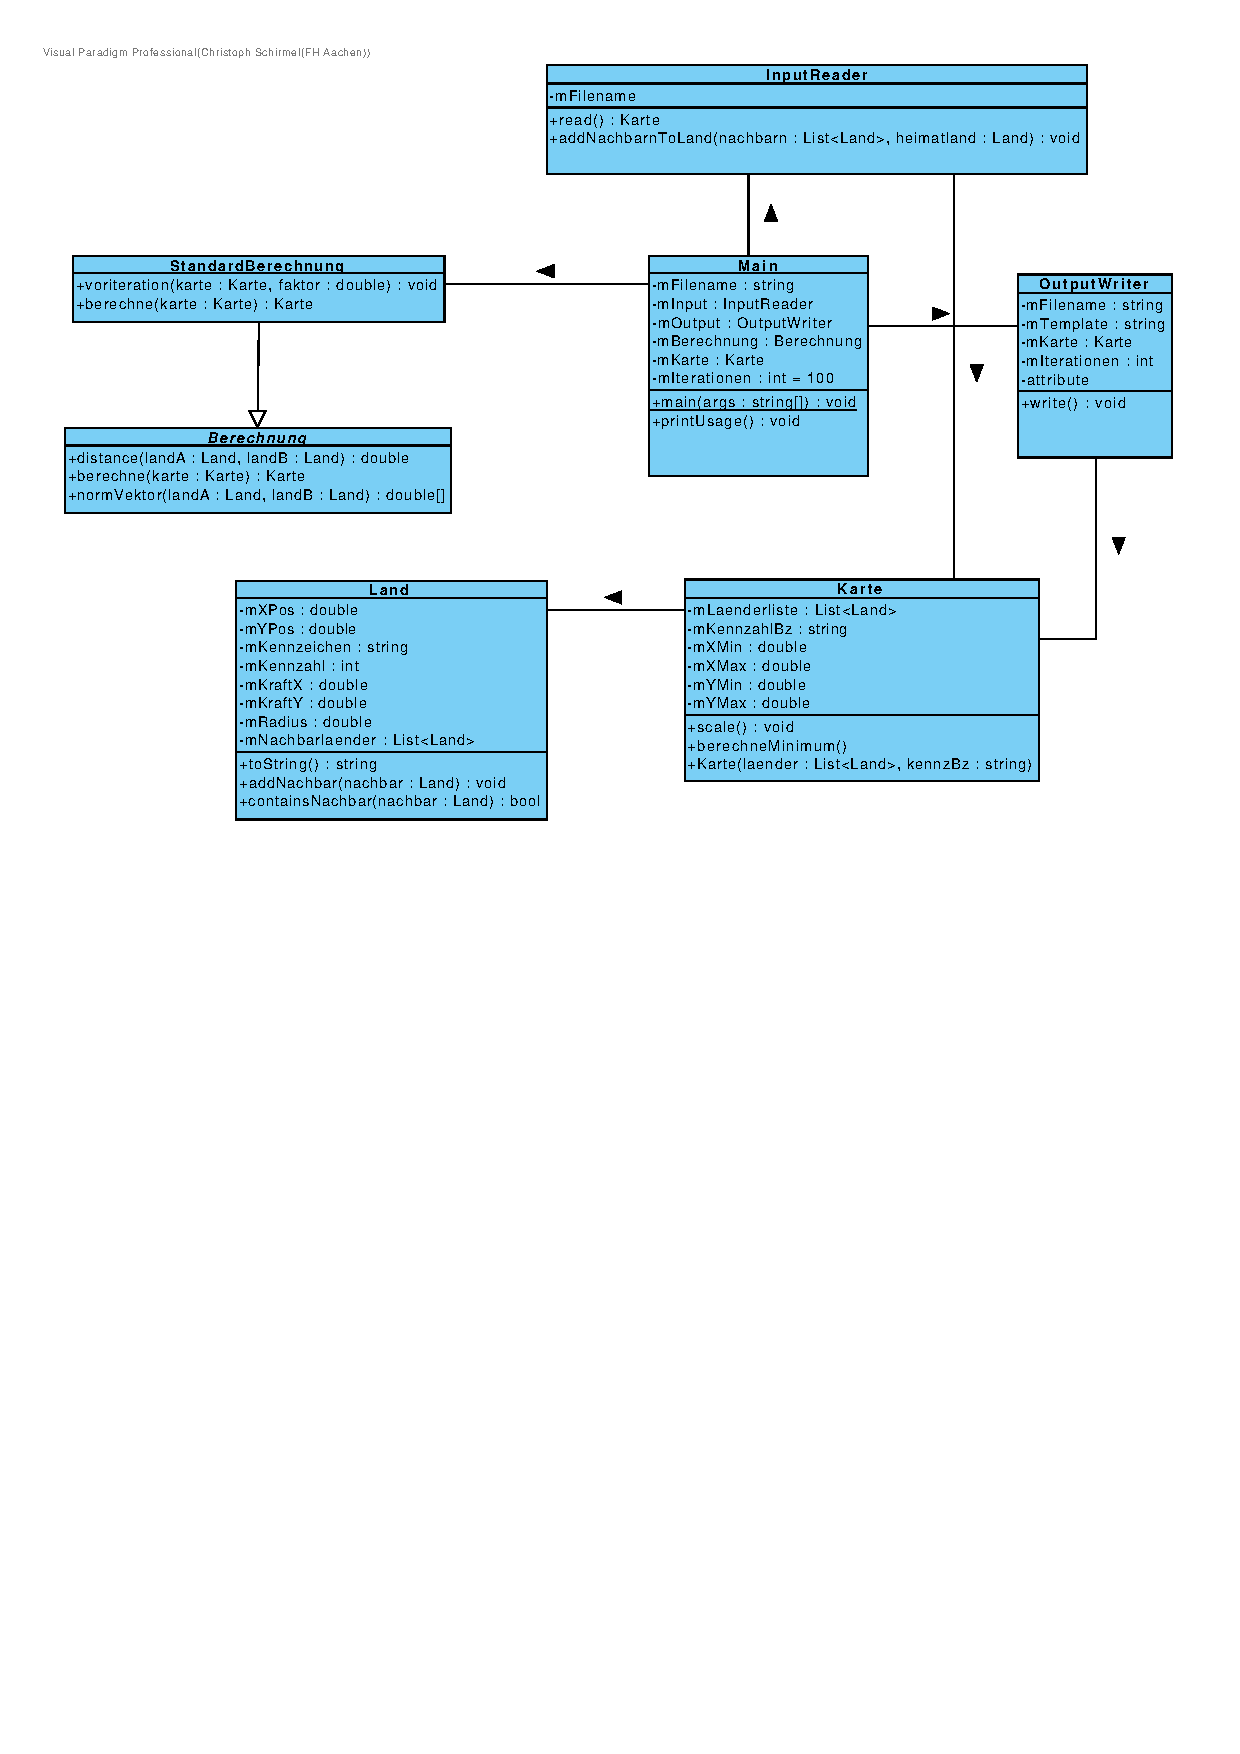
\includegraphics[width=\linewidth]{klassendiagramm_gropro.pdf}

\subsection{Beschreibung}

\subsection{Ablauf Eingabe}

\subsection{Ablauf Ausgabe}

\subsection{Ablauf Hauptalgorithmus}

\subsubsection{TODO}

\subsection{Sequenzdiagramm}

\section{\"Anderungen zum Montagsteil}

\subsection{\"Anderungen in der Klassenstruktur}

\subsection{\"Anderungen beim Algorithmus}

\section{Zusammenfassung und Ausblick}


Zusammenfassung: Läuft.

Ausblick-Ideen: GUI, Parallelisierung, weitere Features


\section{Benutzeranleitung}
\subsection{Ordnerstruktur}
Die .zip Datei beinhaltet die Sourcen, das ausf\"uhrbare Programm, Testskript und diese Dokumentation. Außerdem sind die Ordner ''docu'' und ''tests'' enthalten. In dem ''docu'' Ordner befindet sich ein Unterordner ''html'', in welche sich die mit doxygen generierte Dokumentation des Codes befindet. Zum Anschauen dieser Dokumentation muss die index.html ge\"offnet werden. In dem tests Ordner befinden sich die Testf\"alle.
\subsection{Voraussetzungen}

Compiler und Umgebungen

Python (mindestens 2.7.15, empfohlen 3.7.3), (installationsskript, testskript) (Python-Software-Foundation-Lizenz)
numpy (berkeley software distribution)
optional: Gnuplot (Gnuplot Copyright)

C++/Java/Python für das Programm

%TODO Version angeben

\subsection{Laufzeitumgebung}

\subsection{Installation}

%if python
Eine Installation ist nicht notwendig, weil das Programm in der Programmiersprache Python entwickelt wurde. Python muss nicht übersetzt werden, da es eine interpretierte Sprache ist, die zur Laufzeit vom Interpreter kompiliert wird.

\subsection{Ausführen des Programms}
F\"ur den Aufruf kann folgender Befehl verwendet werden:
python Main.py -i INPUT [-n ITERATIONEN | -s Skalierungsfaktor | -o OUTPUT]


\subsubsection{Direkt}

\subsubsection{Mit dem Skript}

\subsection{Restriktionen beim Dateinamen}
Die Datei muss dem benutzten Betriebssystem entsprechend einen g\"ultigen Dateinamen besitzen.
Sie kann sowohl \"uber den relativen Pfad ausgehend vom Ordner des Aufrufs als auch \"uber den absoluten Pfad angegeben werden.
Die Pfade m\"ussen auch dem Format des benutzten Betriebssystem entsprechen.
Beispiele:
Windows: python \glqq C:$\backslash$Users$\backslash$\grqq{}
Linux: python /home/user/documents/gropro/Main.py

\subsection{Anmerkung}

\section{Tests}

\subsection{IHK Tests}

\subsubsection{IHK Example 01 etc.}

\subsection{Funktionierende Tests}

\subsubsection{F01 bliblablub etc.}

\subsection{Syntax-Fehler Tests}

\subsubsection{S01 lirumlarum}

\subsection{Logik Fehler Tests}

\subsubsection{L01 loremipsum}

\subsection{Optional: Code Coverage Tests, Performance o.ae}

\section{Source-Code}
\subsection{Datei.x}


\lstset{
	basicstyle=\scriptsize\ttfamily,
	language=c++,
	frame=tb,
	tabsize=4,
	showstringspaces=false,
	numbers=left,
	commentstyle=\color{commentgreen},
	keywordstyle=\color{blue},
	stringstyle=\color{orange},
	breaklines=true
}

\section{Code}
\subsection{main.cpp}
%\lstinputlisting[language=c++]{../main.cpp}
\end{document}
